% Options for packages loaded elsewhere
\PassOptionsToPackage{unicode}{hyperref}
\PassOptionsToPackage{hyphens}{url}
\PassOptionsToPackage{dvipsnames,svgnames,x11names}{xcolor}
%
\documentclass[
]{scrreprt}
\usepackage{amsmath,amssymb}
\usepackage{lmodern}
\usepackage{iftex}
\ifPDFTeX
  \usepackage[T1]{fontenc}
  \usepackage[utf8]{inputenc}
  \usepackage{textcomp} % provide euro and other symbols
\else % if luatex or xetex
  \usepackage{unicode-math}
  \defaultfontfeatures{Scale=MatchLowercase}
  \defaultfontfeatures[\rmfamily]{Ligatures=TeX,Scale=1}
  \setmonofont[Scale=0.7]{JuliaMono}
\fi
% Use upquote if available, for straight quotes in verbatim environments
\IfFileExists{upquote.sty}{\usepackage{upquote}}{}
\IfFileExists{microtype.sty}{% use microtype if available
  \usepackage[]{microtype}
  \UseMicrotypeSet[protrusion]{basicmath} % disable protrusion for tt fonts
}{}
\makeatletter
\@ifundefined{KOMAClassName}{% if non-KOMA class
  \IfFileExists{parskip.sty}{%
    \usepackage{parskip}
  }{% else
    \setlength{\parindent}{0pt}
    \setlength{\parskip}{6pt plus 2pt minus 1pt}}
}{% if KOMA class
  \KOMAoptions{parskip=half}}
\makeatother
\usepackage{xcolor}
\IfFileExists{xurl.sty}{\usepackage{xurl}}{} % add URL line breaks if available
\IfFileExists{bookmark.sty}{\usepackage{bookmark}}{\usepackage{hyperref}}
\hypersetup{
  pdftitle={Análisis exploratorio},
  pdfauthor={Andrés Millán; Paula Villanueva},
  colorlinks=true,
  linkcolor={Maroon},
  filecolor={Maroon},
  citecolor={Blue},
  urlcolor={blue},
  pdfcreator={LaTeX via pandoc}}
\urlstyle{same} % disable monospaced font for URLs
\usepackage[top=1.5in,bottom=1in,right=1in,left=1in]{geometry}
\usepackage{color}
\usepackage{fancyvrb}
\newcommand{\VerbBar}{|}
\newcommand{\VERB}{\Verb[commandchars=\\\{\}]}
\DefineVerbatimEnvironment{Highlighting}{Verbatim}{commandchars=\\\{\}}
% Add ',fontsize=\small' for more characters per line
\usepackage{framed}
\definecolor{shadecolor}{RGB}{248,248,248}
\newenvironment{Shaded}{\begin{snugshade}}{\end{snugshade}}
\newcommand{\AlertTok}[1]{\textcolor[rgb]{0.94,0.16,0.16}{#1}}
\newcommand{\AnnotationTok}[1]{\textcolor[rgb]{0.56,0.35,0.01}{\textbf{\textit{#1}}}}
\newcommand{\AttributeTok}[1]{\textcolor[rgb]{0.77,0.63,0.00}{#1}}
\newcommand{\BaseNTok}[1]{\textcolor[rgb]{0.00,0.00,0.81}{#1}}
\newcommand{\BuiltInTok}[1]{#1}
\newcommand{\CharTok}[1]{\textcolor[rgb]{0.31,0.60,0.02}{#1}}
\newcommand{\CommentTok}[1]{\textcolor[rgb]{0.56,0.35,0.01}{\textit{#1}}}
\newcommand{\CommentVarTok}[1]{\textcolor[rgb]{0.56,0.35,0.01}{\textbf{\textit{#1}}}}
\newcommand{\ConstantTok}[1]{\textcolor[rgb]{0.00,0.00,0.00}{#1}}
\newcommand{\ControlFlowTok}[1]{\textcolor[rgb]{0.13,0.29,0.53}{\textbf{#1}}}
\newcommand{\DataTypeTok}[1]{\textcolor[rgb]{0.13,0.29,0.53}{#1}}
\newcommand{\DecValTok}[1]{\textcolor[rgb]{0.00,0.00,0.81}{#1}}
\newcommand{\DocumentationTok}[1]{\textcolor[rgb]{0.56,0.35,0.01}{\textbf{\textit{#1}}}}
\newcommand{\ErrorTok}[1]{\textcolor[rgb]{0.64,0.00,0.00}{\textbf{#1}}}
\newcommand{\ExtensionTok}[1]{#1}
\newcommand{\FloatTok}[1]{\textcolor[rgb]{0.00,0.00,0.81}{#1}}
\newcommand{\FunctionTok}[1]{\textcolor[rgb]{0.00,0.00,0.00}{#1}}
\newcommand{\ImportTok}[1]{#1}
\newcommand{\InformationTok}[1]{\textcolor[rgb]{0.56,0.35,0.01}{\textbf{\textit{#1}}}}
\newcommand{\KeywordTok}[1]{\textcolor[rgb]{0.13,0.29,0.53}{\textbf{#1}}}
\newcommand{\NormalTok}[1]{#1}
\newcommand{\OperatorTok}[1]{\textcolor[rgb]{0.81,0.36,0.00}{\textbf{#1}}}
\newcommand{\OtherTok}[1]{\textcolor[rgb]{0.56,0.35,0.01}{#1}}
\newcommand{\PreprocessorTok}[1]{\textcolor[rgb]{0.56,0.35,0.01}{\textit{#1}}}
\newcommand{\RegionMarkerTok}[1]{#1}
\newcommand{\SpecialCharTok}[1]{\textcolor[rgb]{0.00,0.00,0.00}{#1}}
\newcommand{\SpecialStringTok}[1]{\textcolor[rgb]{0.31,0.60,0.02}{#1}}
\newcommand{\StringTok}[1]{\textcolor[rgb]{0.31,0.60,0.02}{#1}}
\newcommand{\VariableTok}[1]{\textcolor[rgb]{0.00,0.00,0.00}{#1}}
\newcommand{\VerbatimStringTok}[1]{\textcolor[rgb]{0.31,0.60,0.02}{#1}}
\newcommand{\WarningTok}[1]{\textcolor[rgb]{0.56,0.35,0.01}{\textbf{\textit{#1}}}}
\usepackage{graphicx}
\makeatletter
\def\maxwidth{\ifdim\Gin@nat@width>\linewidth\linewidth\else\Gin@nat@width\fi}
\def\maxheight{\ifdim\Gin@nat@height>\textheight\textheight\else\Gin@nat@height\fi}
\makeatother
% Scale images if necessary, so that they will not overflow the page
% margins by default, and it is still possible to overwrite the defaults
% using explicit options in \includegraphics[width, height, ...]{}
\setkeys{Gin}{width=\maxwidth,height=\maxheight,keepaspectratio}
% Set default figure placement to htbp
\makeatletter
\def\fps@figure{htbp}
\makeatother
\setlength{\emergencystretch}{3em} % prevent overfull lines
\providecommand{\tightlist}{%
  \setlength{\itemsep}{0pt}\setlength{\parskip}{0pt}}
\setcounter{secnumdepth}{5}
\usepackage{fvextra}
\DefineVerbatimEnvironment{Highlighting}{Verbatim}{breaklines,commandchars=\\\{\}}
\ifLuaTeX
  \usepackage{selnolig}  % disable illegal ligatures
\fi

\title{Análisis exploratorio}
\author{Andrés Millán \and Paula Villanueva}
\date{03 enero, 2022}

\begin{document}
\maketitle

{
\hypersetup{linkcolor=}
\setcounter{tocdepth}{2}
\tableofcontents
}
\hypertarget{abstract}{%
\chapter{Abstract}\label{abstract}}

Se ha realizado un análisis exploratorio de un conjunto de datos. Este
dataset recoge 8 indicadores económicos de 13 empresas. Tras estudiar la
información recogida en el conjunto, tratando posibles valores perdidos
y outliers, se han aplicado dos tipos de técnicas:

\begin{itemize}
\tightlist
\item
  \textbf{Análisis univariante numérico y gráfico}. En él, se ha
  elaborado un análisis descriptivo numérico clásico y un análisis de
  supuesto de normalidad.
\item
  \textbf{Técnicas multivariantes}: se ha estudiado la correlación entre
  variables, la reducción de la dimensión mediante variables observables
  y latentes. Además, se ha estudiado la normalidad multivariante de los
  datos.
\end{itemize}

Finalmente, se ha construido un clasificador basado en clustering no
jerárquico con el fin de estudiar cómo se agrupan las diferentes
empresas. Descubrimos que existen 4 grupos diferentes.

\hypertarget{introducciuxf3n}{%
\chapter{Introducción}\label{introducciuxf3n}}

Se ha realizado el análisis exploratorio de los datos contenidos en la
base de datos \texttt{DB\_2}. Esta base de datos contiene un grupo
constituido por 13 empresas que se ha clasificado según las puntuaciones
obtenidas en 8 indicadores económicos.

Primero, se ha limpiado el dataset de cualquier anomalía posible. Hemos
encontrado una instancia probablemente errónea, que contenía valores
perdidos e indicadores sin ningún sentido. A continuación, se ha
realizado un análisis descriptivo numérico clásico, esto es, se han
obtenido las medidas de tendencia central, los cuartiles, el coeficiente
de simetría, la dispersión, etc. Además, se han estudiado posibles
outliers. Se ha comprobado también la normalidad de las variables
individualmente mediante gráficos de normalidad.

Una vez preparado el conjunto inicial, procedemos a realizar el análisis
exploratorio multivariante. Se comprobó la correlación entre las
variables mediante un test de Bartlett. A continuación, se realizó un
estudio de la posibilidad de reducción de la dimensión mediante
variables observables, en cuyo caso se ha elegido el número óptimo de
componentes principales usando distintas técnicas gráficas, y mediante
variables latentes, en cuyo caso se ha elegido el número óptimo de
factores a considerar. Lo siguiente fue analizar la normalidad
multivariante de los datos con los tests con el paquete MVN.

Finalmente, para completar nuestro objetivo, se ha realizado un análisis
cluster, es decir, un agrupamiento de los objetos formando clusters de
objetos con un alto grado de homogeneidad interna y heterogeneidad. En
concreto, se ha utilizado el método de las k medias, un método no
jerárquico.

\hypertarget{materiales-y-muxe9todos}{%
\chapter{Materiales y métodos}\label{materiales-y-muxe9todos}}

\hypertarget{materiales}{%
\section{Materiales}\label{materiales}}

La base de datos elegida contiene un grupo constituido por 13 empresas
que se ha clasificado según las puntuaciones obtenidas en 8 indicadores
económicos:

\begin{itemize}
\tightlist
\item
  X1: Indicador de volumen de facturación.
\item
  X2: Indicador de nivel de nueva contratación.
\item
  X3: Indicador del total de clientes.
\item
  X4: Indicador de beneficios de la empresa .
\item
  X5: Indicador de retribución salarial de los empleados.
\item
  X6: Indicador de organización empresarial dentro de la empresa.
\item
  X7: Indicador de relaciones con otras empresas.
\item
  X8: Indicador de nivel de equipamiento (ordenadores, maquinaria,
  etc\ldots).
\end{itemize}

A continuación se muestra una tabla con los estadísticos descriptivos
básicos.

\begin{verbatim}
##        x1               x2                x3               x4                x5               x6               x7               x8        
##  Min.   : 0.128   Min.   : 0.9444   Min.   : 2.167   Min.   : 0.0299   Min.   : 2.557   Min.   : 6.135   Min.   : 1.064   Min.   : 3.949  
##  1st Qu.: 2.476   1st Qu.: 8.6931   1st Qu.: 8.667   1st Qu.: 4.0673   1st Qu.: 3.525   1st Qu.:10.170   1st Qu.: 3.982   1st Qu.: 6.833  
##  Median : 7.584   Median :14.8487   Median :15.167   Median : 5.4044   Median : 5.336   Median :11.374   Median : 5.584   Median : 8.103  
##  Mean   : 6.957   Mean   :14.9138   Mean   :15.167   Mean   : 5.3976   Mean   : 5.107   Mean   :21.006   Mean   : 6.598   Mean   :13.074  
##  3rd Qu.:10.734   3rd Qu.:21.7262   3rd Qu.:21.667   3rd Qu.: 6.5147   3rd Qu.: 5.874   3rd Qu.:31.586   3rd Qu.:10.160   3rd Qu.:20.154  
##  Max.   :14.364   Max.   :25.4261   Max.   :28.167   Max.   :11.3959   Max.   :10.037   Max.   :43.278   Max.   :12.374   Max.   :26.571
\end{verbatim}

\begin{verbatim}
##        x1        x2        x3        x4        x5        x6        x7        x8 
##  4.545099  8.162600  8.437954  2.823818  1.991911 13.779784  4.030662  8.249730
\end{verbatim}

En la siguiente gráfica se muestran los diagramas de cajas de las
variables.

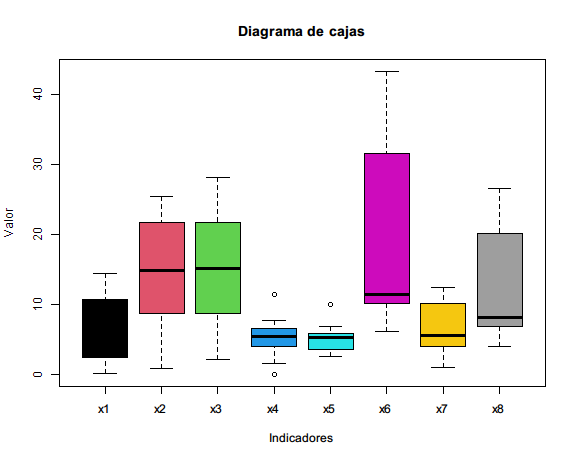
\includegraphics{Entrega_files/figure-latex/unnamed-chunk-4-1.pdf}

\hypertarget{muxe9todos-estaduxedsticos}{%
\section{Métodos estadísticos}\label{muxe9todos-estaduxedsticos}}

En este apartado se indican las distintas técnicas estadísticas que se
han utilizado.

Primero, se ha realizado un análisis numérico y gráfico de cada
variable. De esta forma, mediante en visionado de la estructura del
archivo de datos, se han estudiado las posibles recodificaciones y
valores perdidos. También se ha realizado un análisis descriptivo
numérico clásico, esto es, usando las funciones \texttt{summary},
\texttt{boxplot} y \texttt{skewness} hemos obtenido las medidas de
tendencia central, dispersión, cuartiles, simetría, etc. Por otra parte,
con la función \texttt{check\_outliers} hemos detectado los posibles
outliers mediante el método de mahalanobis. Para comprobar el supuesto
de normalidad, hemos utilizado \texttt{colMeans} y para normalizar los
datos hemos usado \texttt{scale}. De esta forma, podemos visualizar la
normalidad con \texttt{qqplot}.

Con respecto al análisis exploratorio multivariante, se ha utilizado el
test de Bartlett, \texttt{cortest.bartlett}, para estudiar la
correlación entre las variables. En cuanto al Análisis de Componentes
Principales, éste se ha realizado con \texttt{prcomp} y se han utilizado
técnicas gráficas, tales como \texttt{ggplot} y \texttt{fviz\_pca}.
Sobre el AF, se han utilizado otras técnicas gráficas, como
\texttt{ggcorrplot}, \texttt{scree}, \texttt{parallel} y
\texttt{diagram}, y \texttt{factanal} para realizar el test de hipótesis
que constrasta si el número de factores es suficiente. Para realizar el
análisis de la normalidad multivariante, se ha utilizado el paquete
\texttt{MVN}. Específicamente, hemos usado dos tests diferentes: el de
Henze-Zirkler y el de Royston.

Finalmente, para realizar el agrupamiento de los objetos, se ha
utilizado la técnica \texttt{kmeans}, variando el número de clusters con
el fin de comprobar cómo se agrupan las empresas.

\hypertarget{resultados}{%
\chapter{Resultados}\label{resultados}}

En este apartado se mostrarán los resultados obtenidos aplicando las
técnicas mencionadas anteriormente.

\hypertarget{anuxe1lisis-exploratorio-univariante}{%
\section{Análisis exploratorio
univariante}\label{anuxe1lisis-exploratorio-univariante}}

Para estudiar nuestro conjunto de datos, podemos obtener el coeficiente
de simetría de la distribución estadística.

\begin{Shaded}
\begin{Highlighting}[]
\FunctionTok{skewness}\NormalTok{(datos)}
\end{Highlighting}
\end{Shaded}

\begin{verbatim}
##            x1            x2            x3            x4            x5            x6            x7            x8 
## -6.571128e-02 -2.178143e-01  2.441493e-16  8.611432e-02  9.539367e-01  4.214678e-01  1.014152e-01  4.874442e-01
\end{verbatim}

Antes de proceder con el PCA y el AF, es necesario tratar los outliers.
Este fue un punto de discusión importante, pues como vimos en la figura
1, se muestran tres outliers en las variables x4, x5. Sin embargo,
utilizando el método de Mahalanobis, encontramos que no se detecta
ninguno:

\begin{Shaded}
\begin{Highlighting}[]
\FunctionTok{check\_outliers}\NormalTok{(datos, }\AttributeTok{method =} \StringTok{"mahalanobis"}\NormalTok{)}
\end{Highlighting}
\end{Shaded}

\begin{verbatim}
## OK: No outliers detected.
\end{verbatim}

Tras normalizar el conjunto de datos, estudiamos cómo se distribuían las
variables, produciendo el siguiente resultado:

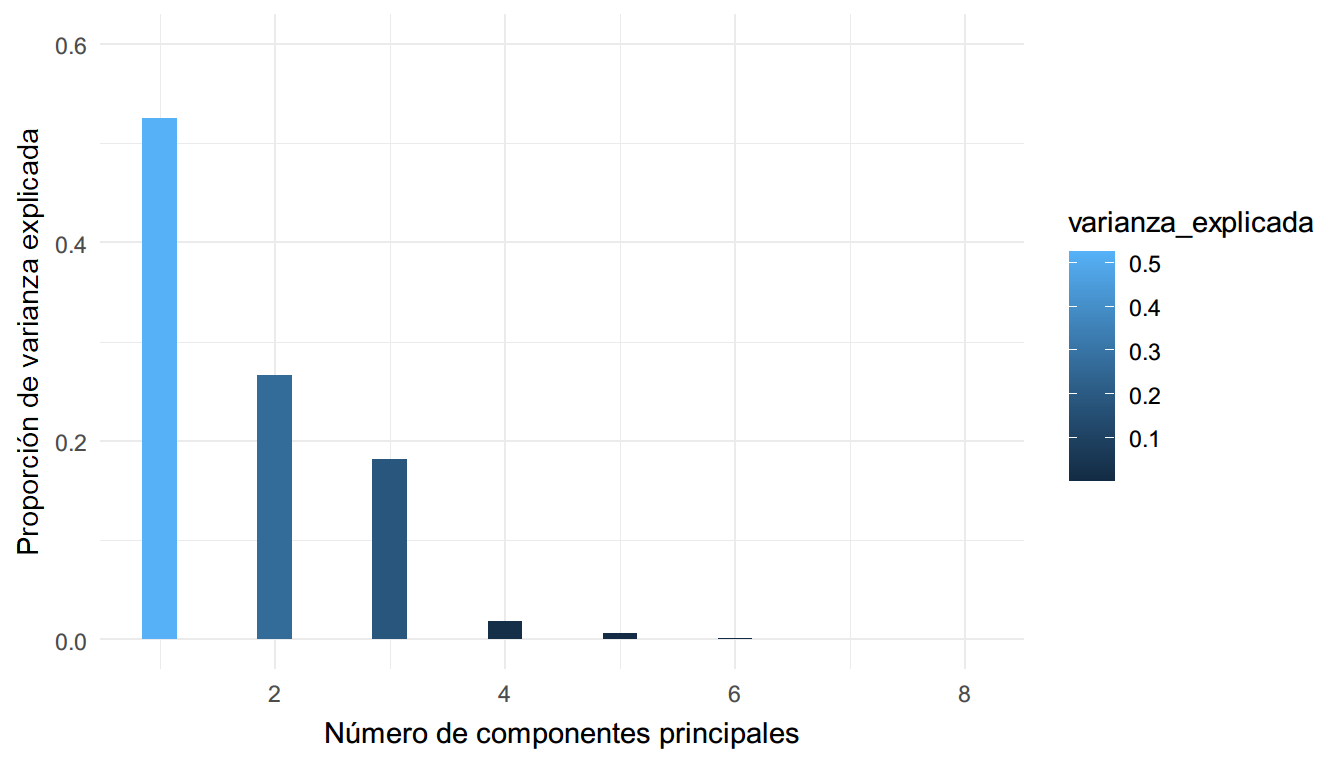
\includegraphics{Entrega_files/figure-latex/unnamed-chunk-7-1.pdf}

\hypertarget{anuxe1lisis-explotatorio-multivariante}{%
\section{Análisis explotatorio
multivariante}\label{anuxe1lisis-explotatorio-multivariante}}

\hypertarget{anuxe1lisis-de-componentes-principales}{%
\subsection{Análisis de componentes
principales}\label{anuxe1lisis-de-componentes-principales}}

Se ha comprobado que existe correlación entre las variables usando el
test de Bartlett, pues obteníamos un \texttt{p-valor} prácticamente
nulo. Esto indica que las variables están correladas, luego procederemos
a realizar un Análisis de Componentes Principales (ACP).

Se han obtenido las desviaciones típicas de cada componente principal y
la proporción de varianza explicada y acumulada. Podemos observar en la
siguiente imagen un análisis gráfico de la varianza explicada.

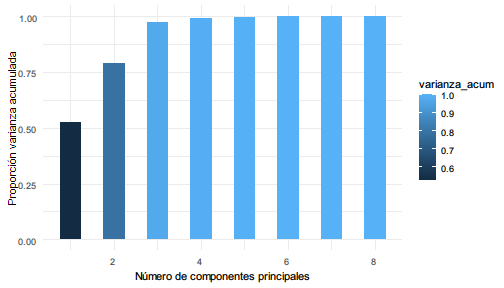
\includegraphics{Entrega_files/figure-latex/unnamed-chunk-8-1.pdf}

De la misma forma, obtenemos un análisis gráfico de la varianza
acumulada.

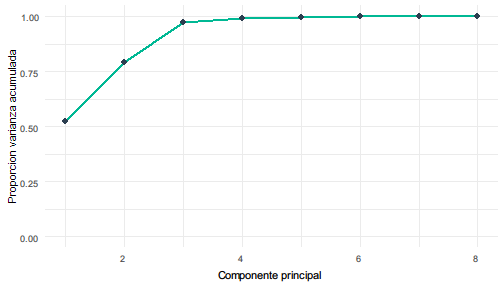
\includegraphics{Entrega_files/figure-latex/unnamed-chunk-9-1.pdf}

A continuación, se seleccionaron el número de componentes principales
óptimo para reducir la dimensión mediante variables observables.
Mediante el método del codo, se ha podido analizar gráficamente y elegir
las componentes principales.

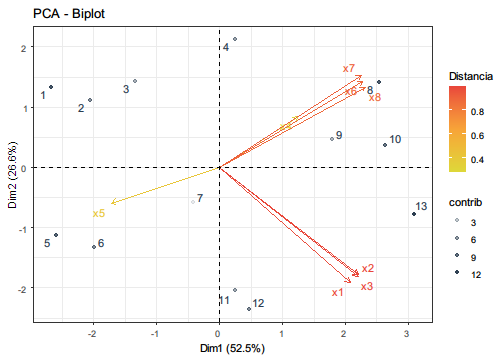
\includegraphics{Entrega_files/figure-latex/unnamed-chunk-10-1.pdf}

En las siguientes gráficas podremos observar la representación conjunta
de variables y observaciones que relaciona visualmente las posibles
relaciones entre las observaciones, las contribuciones de los individuos
a las varianzas de las componentes y el peso de las variables en cada
componentes principal.

Variables y observaciones en la primera y segunda componente principal:

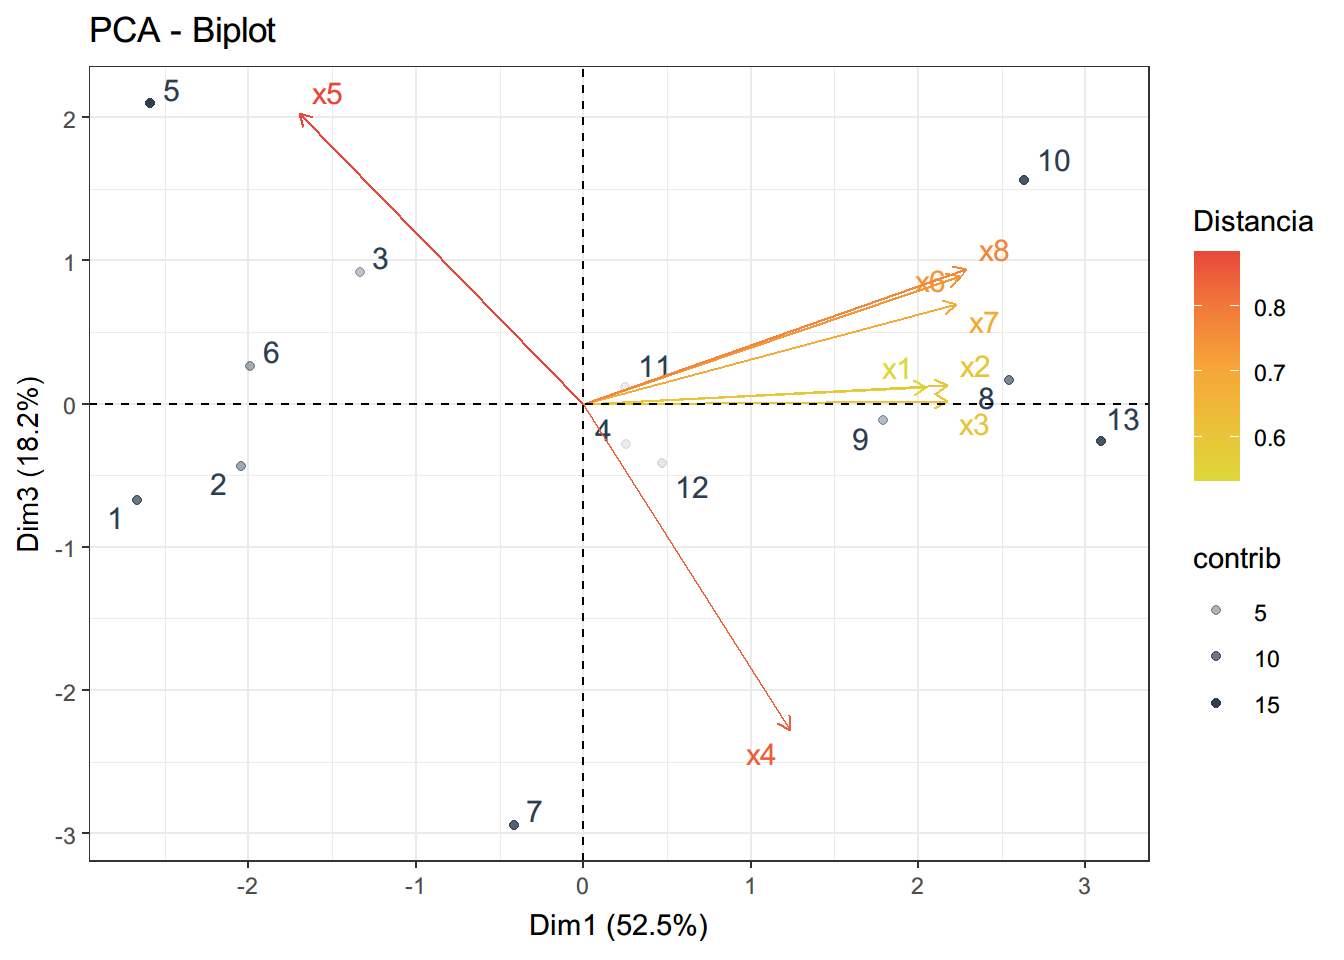
\includegraphics{Entrega_files/figure-latex/unnamed-chunk-11-1.pdf}

Variables y observaciones en la primera y tercera componente principal:

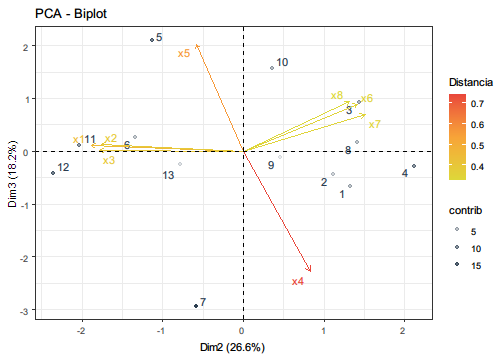
\includegraphics{Entrega_files/figure-latex/unnamed-chunk-12-1.pdf}

Variables y observaciones en la segunda y tercera componente principal:

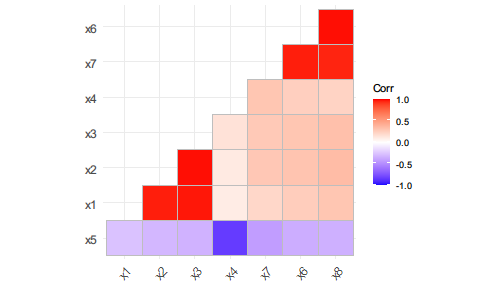
\includegraphics{Entrega_files/figure-latex/unnamed-chunk-13-1.pdf}

\hypertarget{anuxe1lisis-factorial}{%
\subsection{Análisis factorial}\label{anuxe1lisis-factorial}}

Tras realizar el ACP, procedemos a realizar el Análisis Factorial (AF),
el cual tiene sentido porque las variables están correladas:

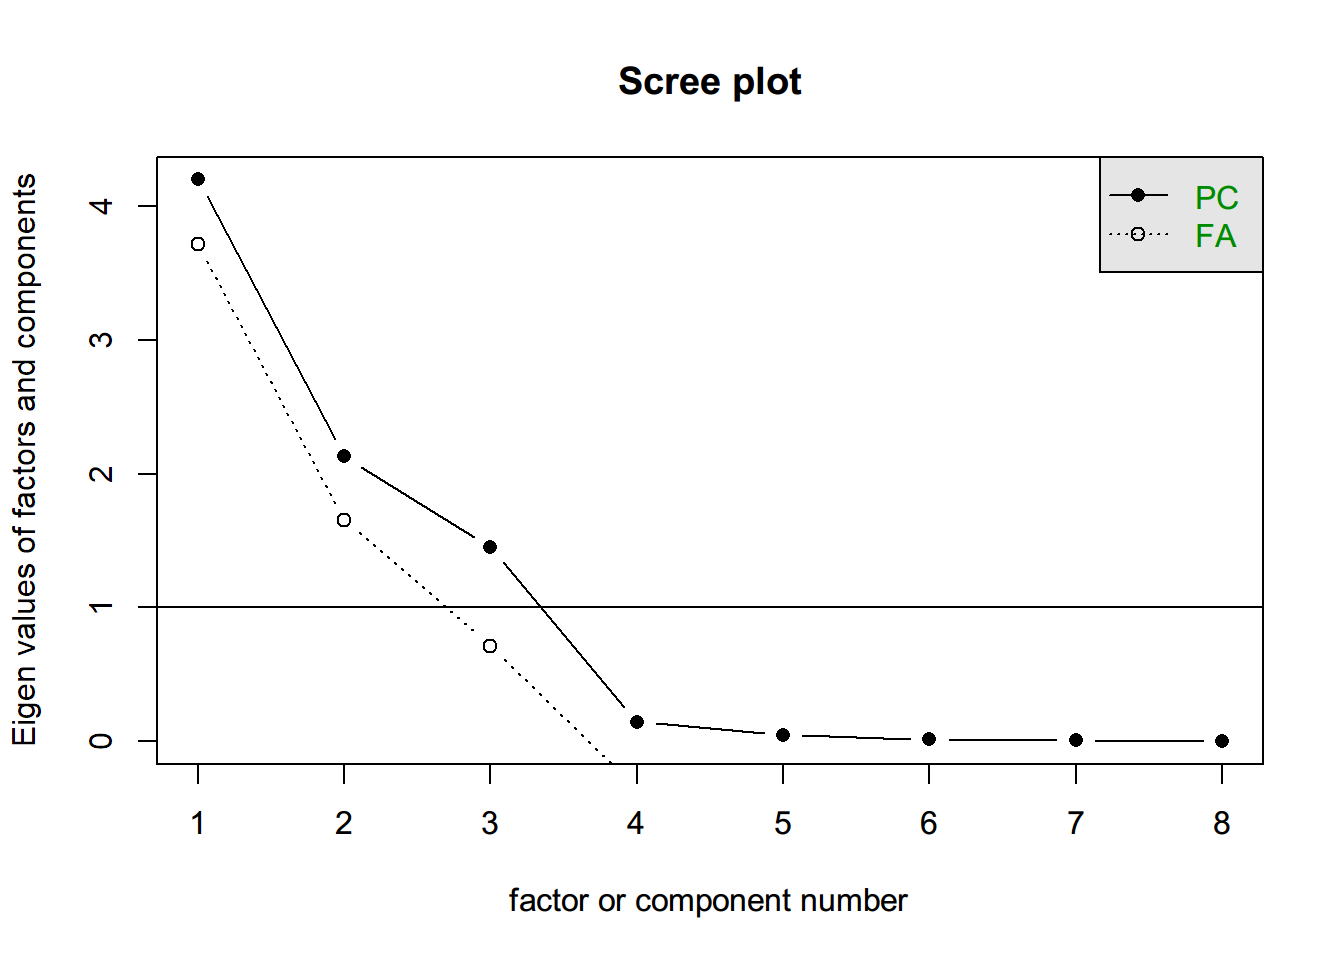
\includegraphics{Entrega_files/figure-latex/unnamed-chunk-14-1.pdf}

Una vez comparadas las salidas con el método del factor principal y con
el de máxima verosimilitud, comparamos las comunalidades y las
unicidades. De esta forma, ya podemos determinar el número óptimo de
factores basándonos en los siguientes gráficos.

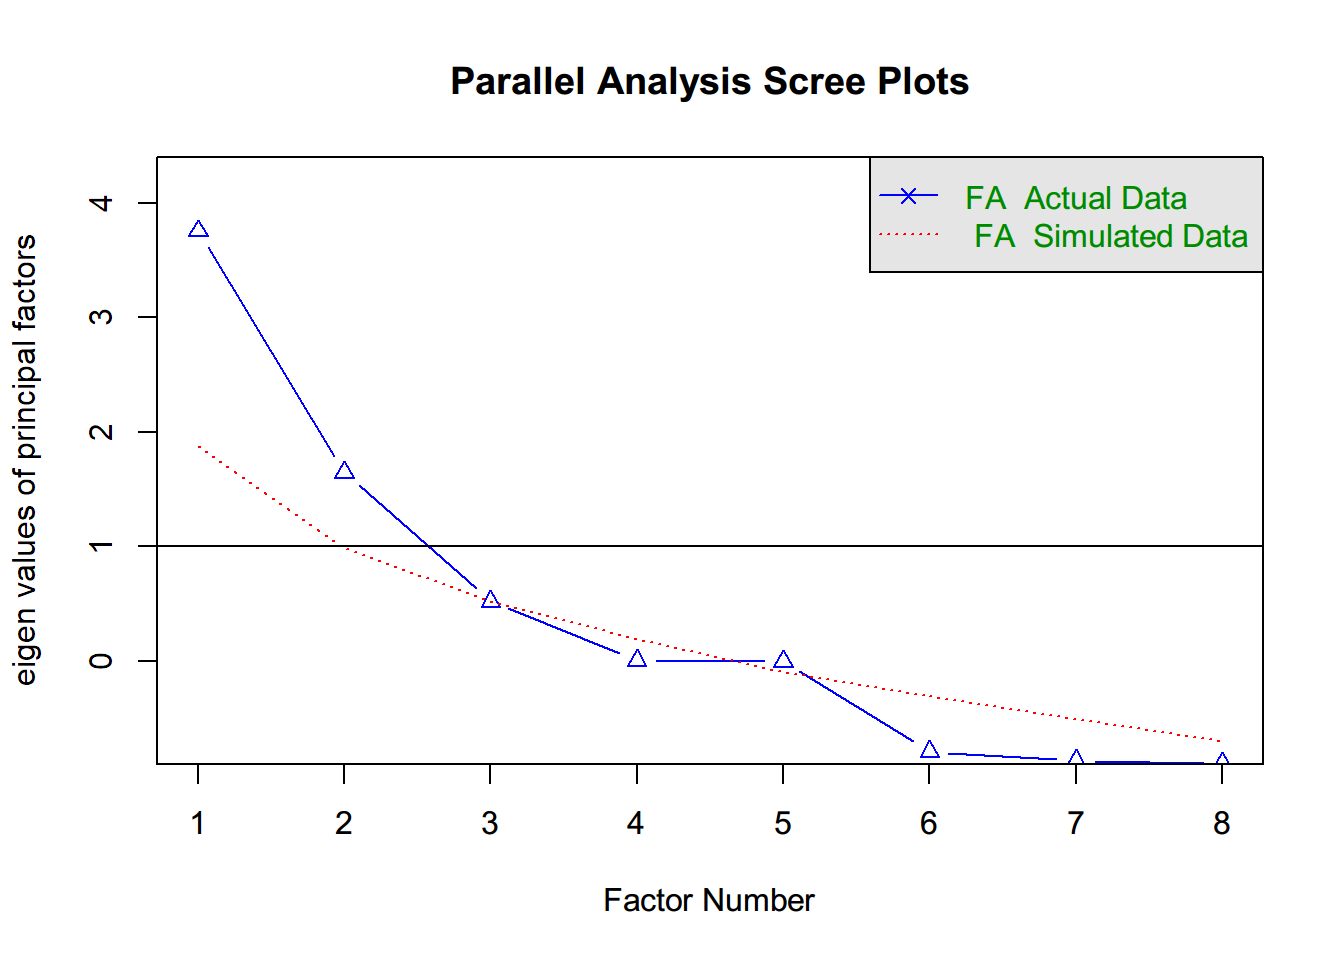
\includegraphics{Entrega_files/figure-latex/unnamed-chunk-15-1.pdf}

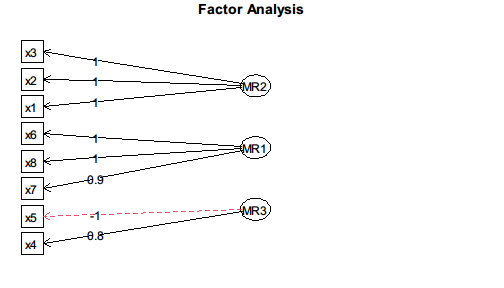
\includegraphics{Entrega_files/figure-latex/unnamed-chunk-16-1.pdf}

\begin{verbatim}
## Parallel analysis suggests that the number of factors =  2  and the number of components =  NA
\end{verbatim}

Estimamos el modelo factorial con 3 factores implementando una rotación
tipo varimax para buscar una interpretación más simple.

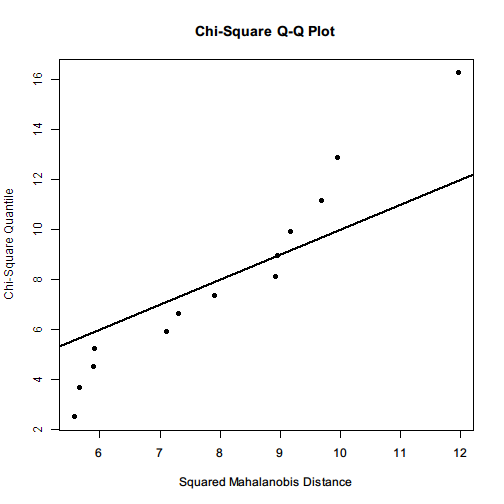
\includegraphics{Entrega_files/figure-latex/unnamed-chunk-17-1.pdf}

Finalmente, con el test de hipótesis contrastamos si el número de
factores es suficiente, lo cual fue cierto.

\hypertarget{anuxe1lisis-de-la-normalidad-multivariante}{%
\subsection{Análisis de la normalidad
multivariante}\label{anuxe1lisis-de-la-normalidad-multivariante}}

Previo al análisis cluster, se ha analizado la normalidad multivariante
de los datos con los tests de Royston y de Henze-Zirkler. Sin embargo
ninguno de los dos tests encuentran evidencias al 5\% de significación
de falta de normalidad multivariante.

Tras realizar el test de Royston, obtenemos la gráfica que se muestra a
continuación.

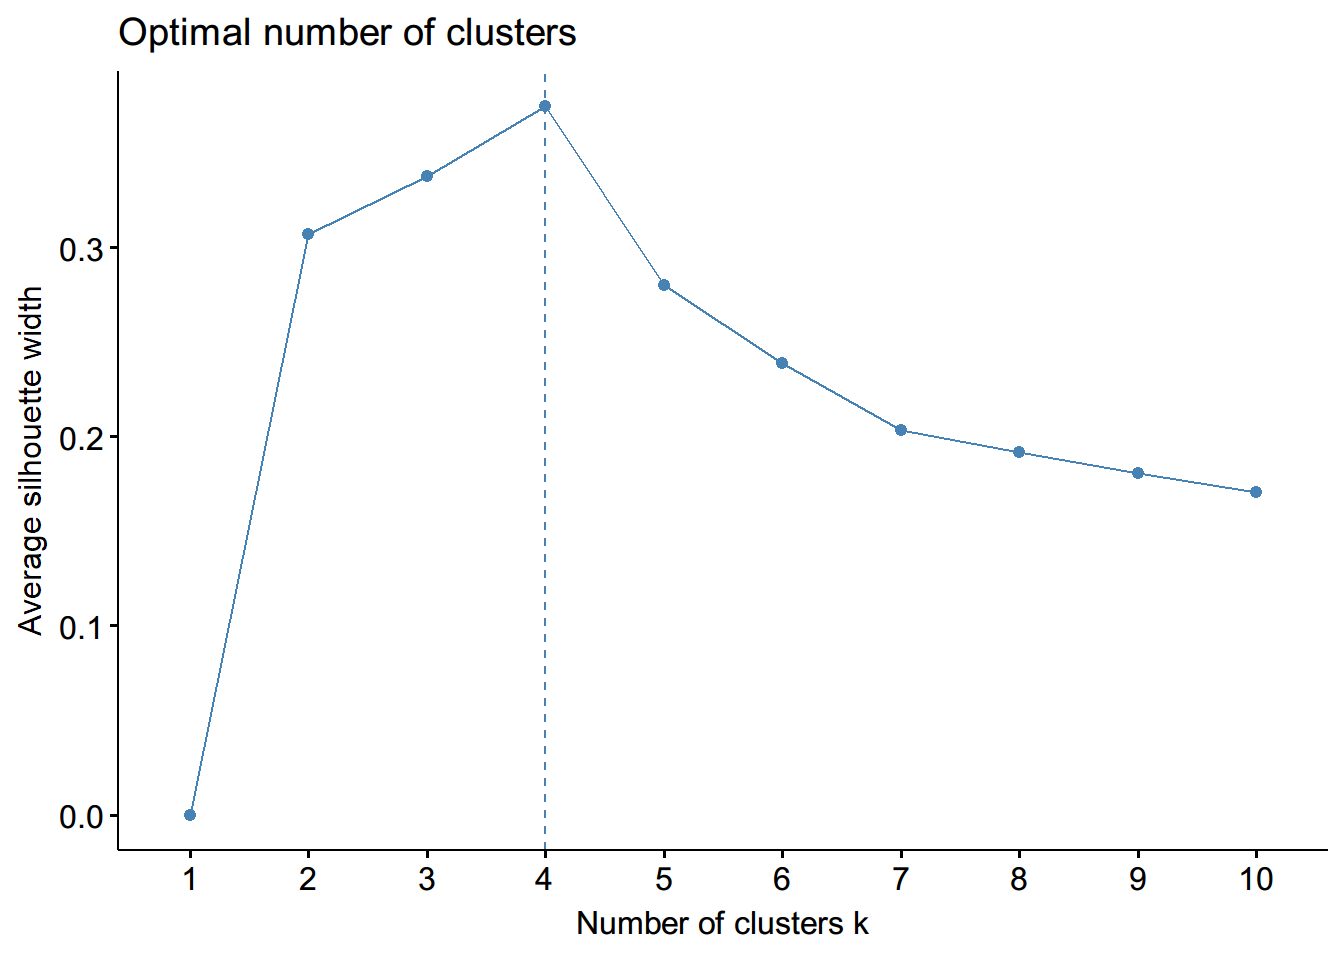
\includegraphics{Entrega_files/figure-latex/unnamed-chunk-18-1.pdf}

\hypertarget{clasificaciuxf3n}{%
\section{Clasificación}\label{clasificaciuxf3n}}

Para finalizar, se han aplicado técnicas de clustering. Hemos llegado a
la conclusión de que el número óptimo de clusters para este dataset es
4:

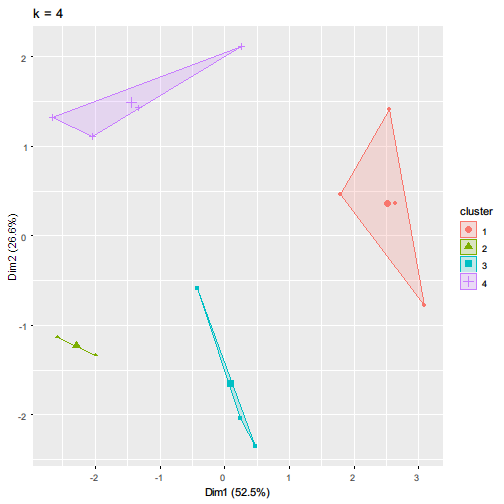
\includegraphics{Entrega_files/figure-latex/unnamed-chunk-19-1.pdf}

K-Means produce las siguientes particiones:

\begin{Shaded}
\begin{Highlighting}[]
\NormalTok{p3}
\end{Highlighting}
\end{Shaded}

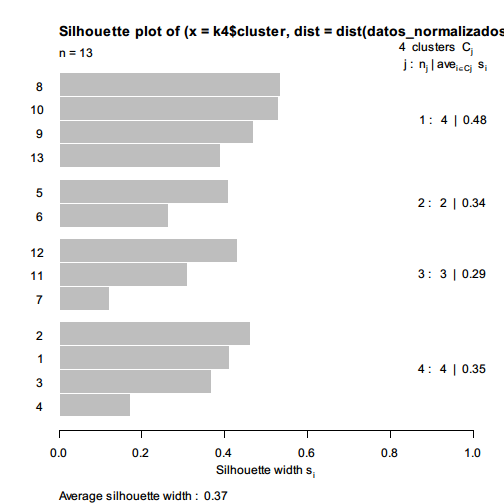
\includegraphics{Entrega_files/figure-latex/unnamed-chunk-20-1.pdf}

Este modelo nos arroja las siguientes siluetas:

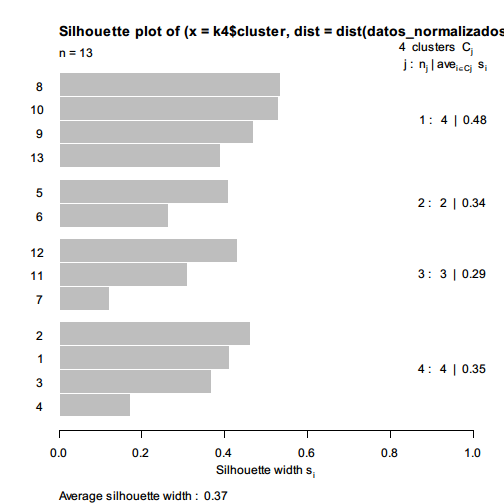
\includegraphics{Entrega_files/figure-latex/unnamed-chunk-21-1.pdf}

\hypertarget{discusiuxf3n-y-conclusiones}{%
\chapter{Discusión y conclusiones}\label{discusiuxf3n-y-conclusiones}}

El objetivo principal consistía en realizar un agrupamiento de los
objetos formando clusters de objetos con un alto grado de homogeneidad
interna y heterogeneidad entre clusters.

En primer lugar, se ha obtenido el coeficiente de simetría de cada
variable en la sección
\protect\hyperlink{Anuxe1lisisux5cux2520exploratorioux5cux2520univariante}{4.1}.
En este problema, hemos obtenido valores positivos o negativos. Un valor
negativo significa que la distribución está sesgada a la derecha,
mientras que un valor positivo indica que la distribución se encuentra
sesgada hacia la izquierda.

Uno de los puntos más controvertidos de este trabajo es la decisión de
eliminar outliers. Como podemos observar en el diagrama de cajas de la
sección \protect\hyperlink{Materiales}{3.1}, se muestran tres outliers
en las variables \texttt{x4} y \texttt{x5}. Sin embargo, se ha tomado la
decisión de no eliminarlos, pues si no fuera así, se ha comprobado que
las métricas de rendimiento bajaban.

Por otra parte, hemos observado que algunas de nuestras variables no se
distribuyen con respecto a una normal. Esto queda evidenciado por la
gráfica de la sección
\protect\hyperlink{Anuxe1lisisux5cux2520exploratorioux5cux2520univariante}{4.1}.
En concreto, las variables x6 y x8 dan problemas. Realizando un test de
shapiro para estas variables, se obtiene lo siguiente:

\begin{verbatim}
## 
##  Shapiro-Wilk normality test
## 
## data:  datos_normalizados[, "x6"]
## W = 0.84811, p-value = 0.02694
\end{verbatim}

\begin{verbatim}
## 
##  Shapiro-Wilk normality test
## 
## data:  datos_normalizados[, "x8"]
## W = 0.86598, p-value = 0.04623
\end{verbatim}

Ambos obtienen un p-valor por debajo de 0.05. Es probable que supongan
una fuente de imprecisiones a la hora de pasar a la distribución normal
multivariante.

En cuanto al Análisis Factorial de la sección
\protect\hyperlink{Anuxe1lisisux5cux2520factorial}{4.2.2}, se ha tomado
la decisión de estimar 3 factores apoyándose en las gráficas obtenidas.
Sin embargo, el análisis paralelo sugería que se estimasen 2 factores,
lo cual produciría
\href{https://v8doc.sas.com/sashtml/stat/chap26/sect21.htm}{un caso de
ultra-Heywood}.

Dos es poco, tres es mucho. Fuente: \url{https://xkcd.com/2560/}

\begin{figure}[H]
\includegraphics[width=0.25\textwidth, height=!]{https://imgs.xkcd.com/comics/confounding_variables.png}
\centering
\caption{mycaption}
\end{figure}

Finalmente, hay otro matiz muy importante que debemos discutir.
\textbf{Nuestro dataset solo tiene 13 instancias}. Hacer un análisis de
calidad con tan pocos datos no es posible. En general, clustering
necesita decenas de instancias como mínimo para producir resultados
realistas.

Para ejemplificar esto, la gráfica de las siluetas. Se genera una
silueta de 0.37, la cual es considerablemente baja. Mirando los
clusters, podemos ver cómo en el cluster 2 existen 2 elementos, mientras
que en el 3 hay 3. Con esto no podemos llegar a ninguna conclusión.

Con el fin de encontrar agrupaciones pertinentes y producir un análisis
de calidad, sería necesario ampliar el número de empresas. De esta
forma, se podrían observar patrones más relevantes.

\hypertarget{distribuciuxf3n-de-las-tareas-entre-las-personas-implicadas}{%
\chapter{Distribución de las tareas entre las personas
implicadas}\label{distribuciuxf3n-de-las-tareas-entre-las-personas-implicadas}}

Para realizar este trabajo, no se han distribuido las tareas, sino que
ambos hemos hecho todas las tareas a la vez, supervisando el uno al otro
y poniendo en común nuestro conocimiento.

\end{document}
